\chapter{Prima esercitazione}
%struttura di partenza
\begin{figure}[htb]
\centering
\begin{tikzpicture}
\scaling{5};
\point{a}{0}{0};
%\point{b}{.5}{0};
\point{c}{1}{0};
\point{d}{2}{.5};
\point{e}{2}{1};
\point{f}{1}{1};
\point{g}{1.12}{1}; %solo per il carrello
\point{h}{1.04}{0.025}; %solo per la cerniera
\point{i}{1.12}{1}; %solo per l'asta che non taglia il carrello
\beam{2}{a}{c}[0][1];
\beam{2}{c}{d}[1][1];
\beam{2}{d}{e}[1][1];
\beam{2}{e}{i}[1][1];
\beam{2}{f}{c}[1][1];
\support{3}{a}[-90]; %incastro % va in senso antiorario
\support{5}{f}[-90]; %molla
\support{2oowh}{g}[-90]; %senza il riempimento sotto
\hinge{1}{h}; %cerniera
\lineload{1}{i}{e}[1][1][.7]; 
\load{1}{d}[90][.8][-1];
\temperature{a}{c}{-.5}{.5}[.5][$+ \Delta T$][$- \Delta T$];
\dimensioning{1}{a}{c}{-1.5}[$l$];
\dimensioning{1}{c}{e}{-1.5}[$l$];
\dimensioning{2}{d}{e}{11.5}[$l/2$];
\dimensioning{2}{c}{d}{11.5}[$l/2$];
\notation{1}{e}{$q$}[above=1.4];
\notation{1}{d}{$F$}[below right];
\notation{1}{f}{$k$}[above left=.6];
\notation{1}{c}{$A$}[below right];
\end{tikzpicture}
\caption{Struttura di partenza}
\end{figure}
Ai valori di $q$, $L$, $k$ e $\Delta T$ sono stati assegnati i valori in modo tale che gli effetti  tensionali di ciascuno di essi fosse confrontabile con quello degli altri. 
Dopo varie prove si sono ottenuti i seguenti valori, con i quali si sono eseguiti tutti i successivi calcoli:
\begin{align*}
	q &= \SI{1000}{\newton \per \metre}\\
	L &= \SI{3000}{\newton}\\
	k &= \SI{100000}{\newton \per \metre}\\
	\Delta T &= \SI{100}{\celsius}
\end{align*}
La sezione delle travi è stata scelta facendo attenzione ad avere una trave snella ovvero avendo una lunghezza pari a $10$ volte lo spessore medio e rispettando la verifica a presso-flessione in campo elastico 
\[
\frac{N}{A} + \frac{M}{W} < \SI{200}{\mega\pascal}
\]
Portando, dopo varie iterazioni, ad avere dei tubi a sezione quadrata con le seguenti caratteristiche
\begin{center}
\begin{minipage}{6cm}
	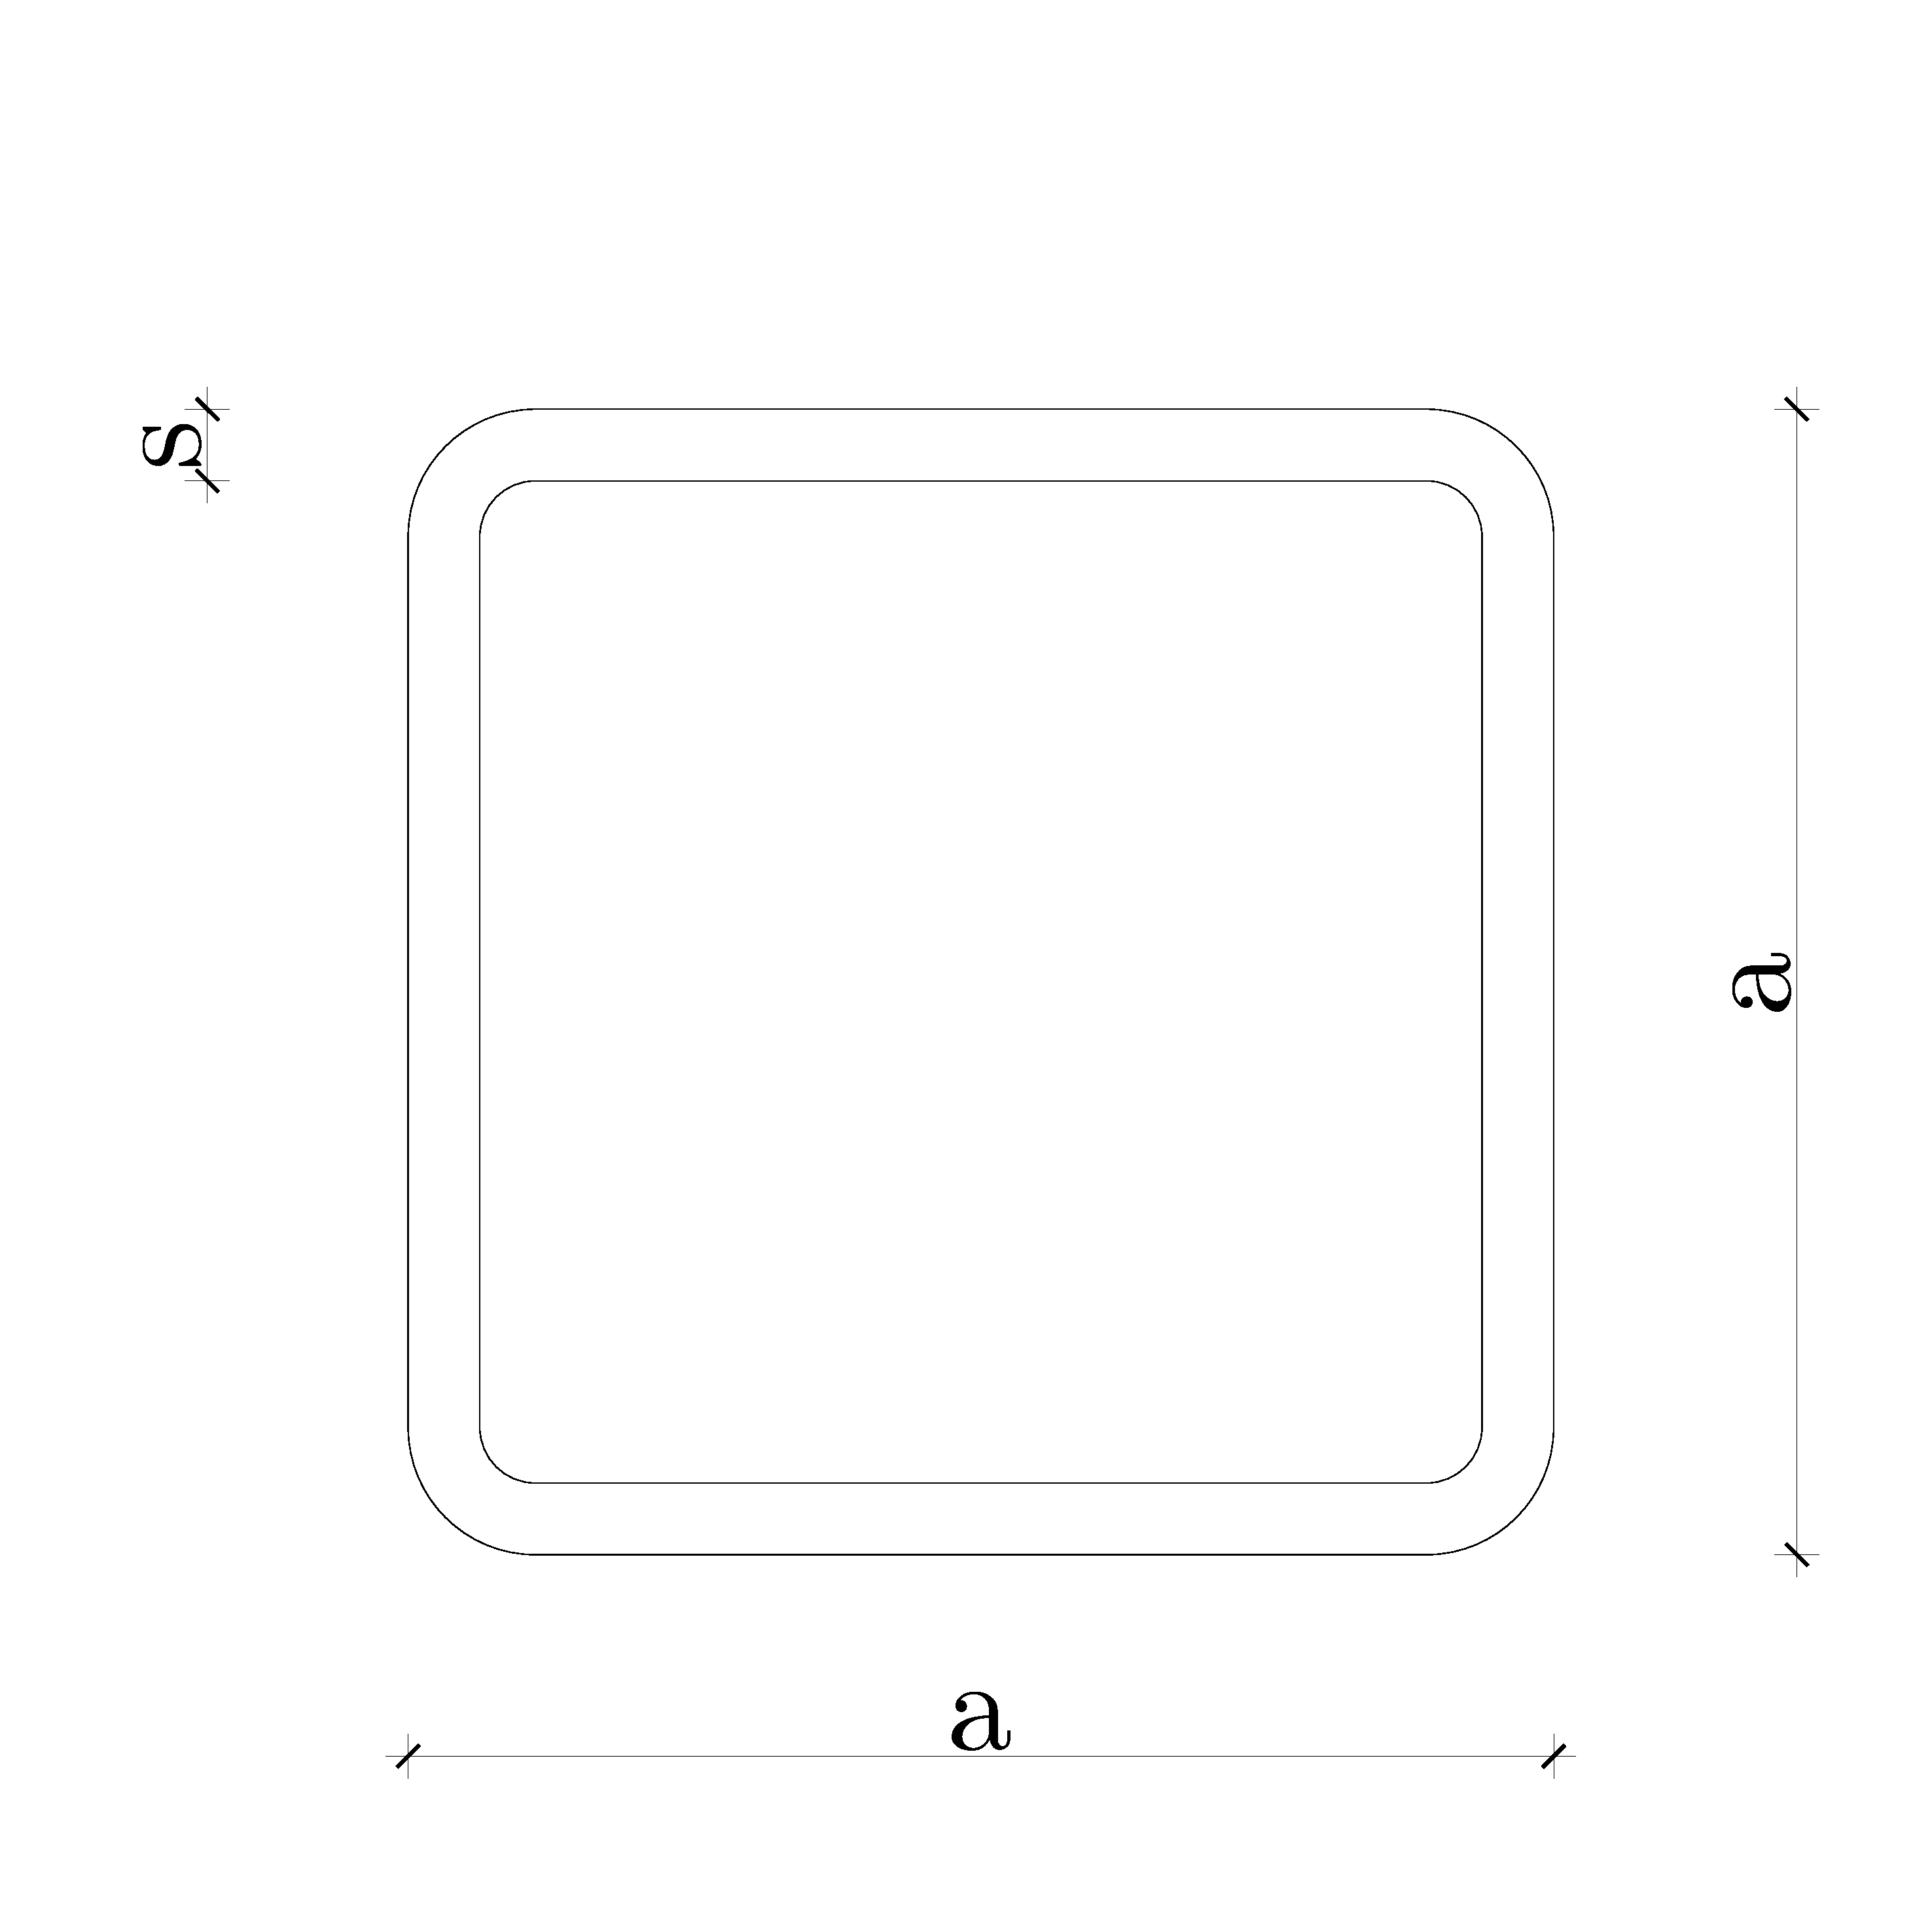
\includegraphics[width=60mm]{img/tubi-quadri.pdf}
\end{minipage}
\begin{minipage}{6cm}
	\begin{align*}
		a &= \SI{200}{\milli\metre}\\
		s &= \SI{6}{\milli\metre}\\
		A &= \SI{46.56}{\centi\metre\squared}\\
		J_X = J_y &= \SI{2923.35}{\centi\metre\tothe{4}}\\
		W_x = W_y &= \SI{292.33}{\centi\metre\cubed}
	\end{align*}
\end{minipage}
\end{center}
%Struttura con i nomi ai punti
\begin{figure}[htb]
\centering
\begin{tikzpicture}
\scaling{5};
\point{a}{0}{0};
%\point{b}{.5}{0};
\point{c}{1}{0};
\point{d}{2}{.5};
\point{e}{2}{1};
\point{f}{1}{1};
\beam{2}{a}{c}[0][1];
\beam{2}{c}{d}[1][1];
\beam{2}{d}{e}[1][1];
\beam{2}{e}{f}[1][1];
\beam{2}{f}{c}[1][1];
\dimensioning{1}{a}{c}{-1.5}[$l$];
\dimensioning{1}{c}{e}{-1.5}[$l$];
\dimensioning{2}{d}{e}{11.5}[$l/2$];
\dimensioning{2}{c}{d}{11.5}[$l/2$];
%disegno assi
\begin{scope}[color=red]
	\load{1}{a}[180][1][-1];
	\load{1}{a}[-90][1][-1];
	\load{1}{c}[180][1][-1];
	\load{1}{c}[-90][1][-1];
	\load{1}{d}[180][1][-1];
	\load{1}{d}[-90][1][-1];
\end{scope}
%nomi aste
\notation{4}{a}{c}[$1$];
\notation{4}{c}{d}[$5$];
\notation{4}{d}{e}[$4$];
\notation{4}{f}{e}[$3$];
\notation{4}{c}{f}[$2$];
%nomi punti
\notation{6}{a}{1};
\notation{6}{c}{2};
\notation{6}{f}{3};
\notation{6}{e}{4};
\notation{6}{d}{5};
\end{tikzpicture}
\caption{Indicazione dei nomi dei nodi e delle aste usati nei calcoli successivi}
\end{figure}
%-----
\section{Analisi tramite PLV}
\e stata degradata la molla bla bla bla
%Diagramma momenti delle strutture 0 e 1
\begin{figure}[htb]
\centering 
\begin{minipage}[b]{0.5\textwidth}
\begin{tikzpicture}
\scaling{3.5};
\point{a}{0}{0};
%\point{b}{.5}{0};
\point{c}{1}{0};
\point{d}{2}{.5};
\point{e}{2}{1};
\point{f}{1}{1};
\point{g}{1.17}{1}; %solo per il carrello
\point{h}{1.04}{0.025}; %solo per la cerniera
\point{i}{1.17}{1}; %solo per l'asta che non taglia il carrello
\beam{2}{a}{c}[0][1];
\beam{2}{c}{d}[1][1];
\beam{2}{d}{e}[1][1];
\beam{2}{e}{i}[1][1];
\beam{2}{f}{c}[1][1];
\support{3}{a}[-90]; % va in senso antiorario
\support{2oowh}{g}[-90]; %senza il riempimento sotto
\hinge{1}{h}; %cerniera
\lineload{1}{i}{e}[1][1][.5];
\load{1}{d}[90][.8][-1];
\notation{1}{e}{$q$}[above=1.4];
\notation{1}{d}{$F$}[below right];
\notation{1}{c}{$A$}[below right];
%diagramma momenti:
\internalforces{a}{c}{-.7}{-.3};
\internalforces{c}{f}{-.3}{0};
\internalforces{c}{d}{0}{.5};
\internalforces{d}{e}{.5}{.3};
\internalforces{e}{g}{.3}{.3};
\end{tikzpicture}
\end{minipage}%
\begin{minipage}[b]{1\textwidth}
\begin{tikzpicture}
\scaling{3.5};
\point{a}{0}{0};
%\point{b}{.5}{0};
\point{c}{1}{0};
\point{d}{2}{.5};
\point{e}{2}{1};
\point{f}{1}{1};
\point{g}{1.17}{1}; %solo per il carrello
\point{h}{1.04}{0.025}; %solo per la cerniera
\point{i}{1.17}{1}; %solo per l'asta che non taglia il carrello
\beam{2}{a}{c}[0][1];
\beam{2}{c}{d}[1][1];
\beam{2}{d}{e}[1][1];
\beam{2}{e}{i}[1][1];
\beam{2}{f}{c}[1][1];
\support{3}{a}[-90]; % va in senso antiorario
\support{2oowh}{g}[-90]; %senza il riempimento sotto
\hinge{1}{h}; %cerniera
\begin{scope}[color=blue]
	\load{1}{f}[180][1][.2];
	\notation{1}{f}{$x_1$}[above left=.2];
\end{scope}
%diagrammi momenti:
\internalforces{a}{c}{-.7}{-.7};
\internalforces{c}{f}{-.7}{0};
\end{tikzpicture}
\end{minipage}%
\caption{Diagramma dei momenti delle strutture (0) e (1)}
\end{figure}
%tabella equazioni:
\begin{table}[H]
\caption{Equazioni dei momenti delle strutture (0) e (1)}
\[
\begin{array}{cccc}
	\toprule
	\textbf{Asta}&\textbf{Lunghezza} & \textbf{Struttura (0)} & \textbf{Struttura (1)}\\
	\midrule
	1&l&\dfrac{7}{2}ql^2-\left(F+ql\right)z&l\\[2ex]
	2&l&\dfrac{7}{2}ql^2-(F+ql)l-\left(F+\dfrac{ql}{2}\right)z &l-z\\
	3&l&\dfrac{qz^2}{2}&0\\[2ex]
	4&\dfrac{l}{2}&\dfrac{ql^2}{2}+\left(\dfrac{ql}{2} + ql\right)z&0\\[2ex]
	5&\sqrt{\dfrac{5}{4}}l&\sqrt{\dfrac{5}{4}}Fz&0\\
	\bottomrule
\end{array}
\]
\end{table}
%Diagramma sforzo normale strutture 0 e 1
\begin{figure}[htb]
\centering 
\begin{minipage}[b]{0.5\textwidth}
\begin{tikzpicture}
\scaling{3.5};
\point{a}{0}{0};
%\point{b}{.5}{0};
\point{c}{1}{0};
\point{d}{2}{.5};
\point{e}{2}{1};
\point{f}{1}{1};
\point{g}{1.17}{1}; %solo per il carrello
\point{h}{1.04}{0.025}; %solo per la cerniera
\point{i}{1.17}{1}; %solo per l'asta che non taglia il carrello
\beam{2}{a}{c}[0][1];
\beam{2}{c}{d}[1][1];
\beam{2}{d}{e}[1][1];
\beam{2}{e}{i}[1][1];
\beam{2}{f}{c}[1][1];
\support{3}{a}[-90]; % va in senso antiorario
\support{2oowh}{g}[-90]; %senza il riempimento sotto
\hinge{1}{h}; %cerniera
\lineload{1}{i}{e}[1][1][.5];
\load{1}{d}[90][.8][-1];
\notation{1}{e}{$q$}[above=1.4];
\notation{1}{d}{$F$}[below right];
\notation{1}{c}{$A$}[below right];
%diagramma N struttura 0:
\internalforces{c}{d}{-.9}{-.9}[0][orange];
\internalforces{d}{e}{.6}{.6}[0][orange];
\internalforces{e}{g}{.3}{.3}[0][orange];
\end{tikzpicture}
\end{minipage}%
\begin{minipage}[b]{1\textwidth}
\begin{tikzpicture}
\scaling{3.5};
\point{a}{0}{0};
%\point{b}{.5}{0};
\point{c}{1}{0};
\point{d}{2}{.5};
\point{e}{2}{1};
\point{f}{1}{1};
\point{g}{1.17}{1}; %solo per il carrello
\point{h}{1.04}{0.025}; %solo per la cerniera
\point{i}{1.17}{1}; %solo per l'asta che non taglia il carrello
\beam{2}{a}{c}[0][1];
\beam{2}{c}{d}[1][1];
\beam{2}{d}{e}[1][1];
\beam{2}{e}{i}[1][1];
\beam{2}{f}{c}[1][1];
\support{3}{a}[-90]; % va in senso antiorario
\support{2oowh}{g}[-90]; %senza il riempimento sotto
\hinge{1}{h}; %cerniera
\begin{scope}[color=blue]
	\load{1}{f}[180][1][.2];
	\notation{1}{f}{$x_1$}[above left=.2];
\end{scope}
%diagrammi N struttura 1:
\internalforces{a}{c}{-.7}{-.7}[0][orange];
\end{tikzpicture}
\end{minipage}%
\caption{Diagramma degli sforzi normali delle strutture (0) e (1)}
\end{figure}
\begin{align*}
	\mathscr{L}_{int} &= \mathscr{L}_{ext}	\\
	\eta_{01}+x_1 \eta_{11} + \eta_T &= - \eta_m V_3 \\
	& \qquad \eta_{01}= \frac{1}{EI}\sum_{k}\int_L m_0 \cdot m_1\\
	& \qquad \eta_{11}= \frac{1}{EI}\sum_{k}\int_L m_1 \cdot m_1\\
	& \qquad \eta_T = \frac{2 \alpha \Delta T}{H}l^2 \\
	& \qquad \eta_m = \frac{1}{k_m} \left( F+\frac{ql}{2}\right)\\
	 \hookrightarrow \quad  x_1 &= \frac{15}{2}ql
\end{align*}
%
\section{Analisi tramite calcolo matriciale}
\section{Analisi tramite FEM}


\begin{sideways}
\begin{minipage}{\textheight}
\[
   \left(
\begin{array}{ccccccccccccccc}
 \frac{8 A \text{EY}}{5 \sqrt{5} L}+\frac{A \text{EY}}{L}+\frac{96 \text{EY}
   \text{IN}}{25 \sqrt{5} L^3}+\frac{12 \text{EY} \text{IN}}{L^3} & \frac{192
   \text{EY} \text{IN}}{25 \sqrt{5} L^3}-\frac{4 A \text{EY}}{5 \sqrt{5} L} &
   \frac{6 \text{EY} \text{IN}}{L^2} & \frac{24 \text{EY} \text{IN}}{5
   \sqrt{5} L^2} & -\frac{12 \text{EY} \text{IN}}{L^3} & 0 & 0 & \frac{6
   \text{EY} \text{IN}}{L^2} & 0 & 0 & 0 & 0 & -\frac{8 A \text{EY}}{5
   \sqrt{5} L}-\frac{96 \text{EY} \text{IN}}{25 \sqrt{5} L^3} & \frac{4 A
   \text{EY}}{5 \sqrt{5} L}-\frac{192 \text{EY} \text{IN}}{25 \sqrt{5} L^3} &
   \frac{24 \text{EY} \text{IN}}{5 \sqrt{5} L^2} \\
 \frac{192 \text{EY} \text{IN}}{25 \sqrt{5} L^3}-\frac{4 A \text{EY}}{5
   \sqrt{5} L} & \frac{2 A \text{EY}}{5 \sqrt{5} L}+\frac{A
   \text{EY}}{L}+\frac{384 \text{EY} \text{IN}}{25 \sqrt{5} L^3}+\frac{12
   \text{EY} \text{IN}}{L^3} & -\frac{6 \text{EY} \text{IN}}{L^2} & \frac{48
   \text{EY} \text{IN}}{5 \sqrt{5} L^2} & 0 & -\frac{A \text{EY}}{L} & 0 & 0 &
   0 & 0 & 0 & 0 & \frac{4 A \text{EY}}{5 \sqrt{5} L}-\frac{192 \text{EY}
   \text{IN}}{25 \sqrt{5} L^3} & -\frac{2 A \text{EY}}{5 \sqrt{5} L}-\frac{384
   \text{EY} \text{IN}}{25 \sqrt{5} L^3} & \frac{48 \text{EY} \text{IN}}{5
   \sqrt{5} L^2} \\
 \frac{6 \text{EY} \text{IN}}{L^2} & -\frac{6 \text{EY} \text{IN}}{L^2} &
   \frac{8 \text{EY} \text{IN}}{L} & 0 & -\frac{6 \text{EY} \text{IN}}{L^2} &
   0 & 0 & \frac{2 \text{EY} \text{IN}}{L} & 0 & 0 & 0 & 0 & 0 & 0 & 0 \\
 \frac{24 \text{EY} \text{IN}}{5 \sqrt{5} L^2} & \frac{48 \text{EY}
   \text{IN}}{5 \sqrt{5} L^2} & 0 & \frac{8 \text{EY} \text{IN}}{\sqrt{5} L} &
   0 & 0 & 0 & 0 & 0 & 0 & 0 & 0 & -\frac{24 \text{EY} \text{IN}}{5 \sqrt{5}
   L^2} & -\frac{48 \text{EY} \text{IN}}{5 \sqrt{5} L^2} & \frac{4 \text{EY}
   \text{IN}}{\sqrt{5} L} \\
 -\frac{12 \text{EY} \text{IN}}{L^3} & 0 & -\frac{6 \text{EY} \text{IN}}{L^2}
   & 0 & \frac{A \text{EY}}{L}+\frac{12 \text{EY} \text{IN}}{L^3}+\text{Km} &
   0 & 0 & -\frac{6 \text{EY} \text{IN}}{L^2} & 0 & -\frac{A \text{EY}}{L} & 0
   & 0 & 0 & 0 & 0 \\
 0 & -\frac{A \text{EY}}{L} & 0 & 0 & 0 & \frac{A \text{EY}}{L} & 0 & 0 & 0 &
   0 & 0 & 0 & 0 & 0 & 0 \\
 0 & 0 & 0 & 0 & 0 & 0 & \frac{12 \text{EY} \text{IN}}{L^3} & 0 & \frac{6
   \text{EY} \text{IN}}{L^2} & 0 & -\frac{12 \text{EY} \text{IN}}{L^3} &
   \frac{6 \text{EY} \text{IN}}{L^2} & 0 & 0 & 0 \\
 \frac{6 \text{EY} \text{IN}}{L^2} & 0 & \frac{2 \text{EY} \text{IN}}{L} & 0 &
   -\frac{6 \text{EY} \text{IN}}{L^2} & 0 & 0 & \frac{4 \text{EY}
   \text{IN}}{L} & 0 & 0 & 0 & 0 & 0 & 0 & 0 \\
 0 & 0 & 0 & 0 & 0 & 0 & \frac{6 \text{EY} \text{IN}}{L^2} & 0 & \frac{4
   \text{EY} \text{IN}}{L} & 0 & -\frac{6 \text{EY} \text{IN}}{L^2} & \frac{2
   \text{EY} \text{IN}}{L} & 0 & 0 & 0 \\
 0 & 0 & 0 & 0 & -\frac{A \text{EY}}{L} & 0 & 0 & 0 & 0 & \frac{A
   \text{EY}}{L}+\frac{96 \text{EY} \text{IN}}{L^3} & 0 & -\frac{24 \text{EY}
   \text{IN}}{L^2} & -\frac{96 \text{EY} \text{IN}}{L^3} & 0 & -\frac{24
   \text{EY} \text{IN}}{L^2} \\
 0 & 0 & 0 & 0 & 0 & 0 & -\frac{12 \text{EY} \text{IN}}{L^3} & 0 & -\frac{6
   \text{EY} \text{IN}}{L^2} & 0 & \frac{2 A \text{EY}}{L}+\frac{12 \text{EY}
   \text{IN}}{L^3} & -\frac{6 \text{EY} \text{IN}}{L^2} & 0 & -\frac{2 A
   \text{EY}}{L} & 0 \\
 0 & 0 & 0 & 0 & 0 & 0 & \frac{6 \text{EY} \text{IN}}{L^2} & 0 & \frac{2
   \text{EY} \text{IN}}{L} & -\frac{24 \text{EY} \text{IN}}{L^2} & -\frac{6
   \text{EY} \text{IN}}{L^2} & \frac{12 \text{EY} \text{IN}}{L} & \frac{24
   \text{EY} \text{IN}}{L^2} & 0 & \frac{4 \text{EY} \text{IN}}{L} \\
 -\frac{8 A \text{EY}}{5 \sqrt{5} L}-\frac{96 \text{EY} \text{IN}}{25 \sqrt{5}
   L^3} & \frac{4 A \text{EY}}{5 \sqrt{5} L}-\frac{192 \text{EY} \text{IN}}{25
   \sqrt{5} L^3} & 0 & -\frac{24 \text{EY} \text{IN}}{5 \sqrt{5} L^2} & 0 & 0
   & 0 & 0 & 0 & -\frac{96 \text{EY} \text{IN}}{L^3} & 0 & \frac{24 \text{EY}
   \text{IN}}{L^2} & \frac{8 A \text{EY}}{5 \sqrt{5} L}+\frac{96 \text{EY}
   \text{IN}}{25 \sqrt{5} L^3}+\frac{96 \text{EY} \text{IN}}{L^3} & \frac{192
   \text{EY} \text{IN}}{25 \sqrt{5} L^3}-\frac{4 A \text{EY}}{5 \sqrt{5} L} &
   \frac{24 \text{EY} \text{IN}}{L^2}-\frac{24 \text{EY} \text{IN}}{5 \sqrt{5}
   L^2} \\
 \frac{4 A \text{EY}}{5 \sqrt{5} L}-\frac{192 \text{EY} \text{IN}}{25 \sqrt{5}
   L^3} & -\frac{2 A \text{EY}}{5 \sqrt{5} L}-\frac{384 \text{EY}
   \text{IN}}{25 \sqrt{5} L^3} & 0 & -\frac{48 \text{EY} \text{IN}}{5 \sqrt{5}
   L^2} & 0 & 0 & 0 & 0 & 0 & 0 & -\frac{2 A \text{EY}}{L} & 0 & \frac{192
   \text{EY} \text{IN}}{25 \sqrt{5} L^3}-\frac{4 A \text{EY}}{5 \sqrt{5} L} &
   \frac{2 A \text{EY}}{5 \sqrt{5} L}+\frac{2 A \text{EY}}{L}+\frac{384
   \text{EY} \text{IN}}{25 \sqrt{5} L^3} & -\frac{48 \text{EY} \text{IN}}{5
   \sqrt{5} L^2} \\
 \frac{24 \text{EY} \text{IN}}{5 \sqrt{5} L^2} & \frac{48 \text{EY}
   \text{IN}}{5 \sqrt{5} L^2} & 0 & \frac{4 \text{EY} \text{IN}}{\sqrt{5} L} &
   0 & 0 & 0 & 0 & 0 & -\frac{24 \text{EY} \text{IN}}{L^2} & 0 & \frac{4
   \text{EY} \text{IN}}{L} & \frac{24 \text{EY} \text{IN}}{L^2}-\frac{24
   \text{EY} \text{IN}}{5 \sqrt{5} L^2} & -\frac{48 \text{EY} \text{IN}}{5
   \sqrt{5} L^2} & \frac{8 \text{EY} \text{IN}}{\sqrt{5} L}+\frac{8 \text{EY}
   \text{IN}}{L} \\
\end{array}
\right)
\]
\end{minipage}
\end{sideways}


\section{Confronto spostamenti in A}
%tabella equazioni:
\begin{table}[H]
\caption{Confronto spostamenti nei nodi}
\centering
\begin{tabular}{cSSS}
	\toprule
	\textbf{Nodo}&\textbf{PLV} & \textbf{Matriciale} & \textbf{FEM}\\
	\midrule
	10 & 1.111& 1.111& 1.111\\	 
	\bottomrule
\end{tabular}
\end{table}
